\chapter{{\LN}}\label{sec:lightning_network}

\section{Introduction}

The \emph{{\LN}} is a peer-to-peer protocol whose aim is to provide a scalable technique for processing Bitcoin micro-transactions. Indeed, Bitcoin has long suffered severe scalability limitations, one of them being related to a strict upper limit on the transaction rate.\\
Therefore, with the awareness that some of these limitations are features in Bitcoin, the {\LN} tries to solve
the scalability problem by offering an \emph{off-chain} solution that enables peers to exchange partially
signed transactions without violating the Bitcoin rules.\\
{\LN} was proposed for the first time in 2015 by Poon and Dryja in  ~\cite{lightning-network-paper},
and then implemented in 2018 with the \emph{c-lightning} (aka \emph{core lightning}) implementation.
However, the protocol is evolving over the years through a process of standardization~~\cite{lightning-bolts}.

\section{Off-Chain Protocol}

The Bitcoin network has scalability problems compared with modern payment system that people use daily.
In particular, these problems are related to the space required by the blockchain to store each transaction,
and the relatively long time that is required to consider a transaction confirmed in the blockchain.

For instance, the Visa payment network  achieved around 65,000 ~\cite{visa-sheet} transactions per second, while
Bitcoin currently supports around 7 transactions per second with a required space estimated of 1 MB per block. Considering
an average of 300 bytes per bitcoin transaction and assuming unlimited block sizes, the space for storing the same number
of transactions is estimated in the order of terabytes ~\cite{lightning-network-paper}. Therefore, in order to use the Bitcoin
protocol as an alternative of the current payment systems for a subset of the problem, such as the accessibility to the modern world
to people that live in not developed countries, there is a need to make the protocol more scalable.

This kind of problem is almost considered a well-studied problem, and different solutions have been proposed, but most of them require a hard fork  of the protocol itself.
One of the most popular hard fork examples is given by Bitcoin Cash, which 
increases the block size to be able to insert inside a block more transactions.
However, in the Bitcoin ecosystem (based on the Bitcoin Core implementation) the idea of an hard fork is considered 
as last resort, and some of the ideas to solve the scalability of the protocol are proposed through 
Bitcoin Script tricks by proposing a soft-fork of the Bitcoin protocol.

\section{{\LN} Basics}

The actual {\LN} is more complicated than the original proposal of  ~\cite{lightning-network-paper}, and it has deeply
evolved from the first time that the paper came out. However, the idea described in the paper was an evolution
of some previous ideas regarding the possibility to have payment channels with Bitcoin, and in this section we will describe the basics of the initial proposal.

\subsection{Payment Channel}

A Payment Channel, also known as Micropayment Channel, is a class of techniques designed to allow users to make multiple
Bitcoin transactions without committing all of the transactions to the Bitcoin blockchain. In a typical payment channel,
only two transactions are added to the blockchain but an unlimited or nearly unlimited number of payments
can be made between the participants.\\
In fact, the concept of replacing an old transaction with the new one is proposed from \emph{Satoshi Nakamoto}
in the mailinglist~~\cite{payment-channels-satoshi}, and
the basic concept to implement this feature was present from the version 0.0.1 of Bitcoin core. However, this solution
was not safe because with this method there is the possibility to steal funds from the other party or parties.\\

Later, there was a new proposal to implement  \emph{Spillman-style payment channels}, and it is
implemented inside  \emph{bitcoinj}~\cite{bitcoinj-impl}. Spillman payment channels are unidirectional, i.e., 
there is a payer and a payee, in this kind of channel it is not possible to transfer money back in the reverse direction, and the payment
channels expire after a specific time.
In addition, the receiver needs to close the channel before the expiration time.
However, this proposal has malleability problems solved later by the \emph{BIP  65}~\cite{bip65} Bitcoin proposal that includes a new Bitcoin Script OP code,
called \emph{OP\_CHECKLOCKTIMEVERIFY}, that unlocks a new version of payment channels called \emph{CLTV-style payment channels}.\\
While the idea of payment channels start to be explored around the Bitcoin community, two new proposals came out:
\emph{Poon-Dryja payment channels}~\cite{lightning-network-paper} (currently used in the {\LN}),
and \emph{Decker-Wattenhofer duplex payment channels}~\cite{Decker2015fast}; these proposals try to improve the known state
of the art by allowing more complex payment channel operations.

In particular, in Poon-Dryja payment channels the funds are locked into a 2-of-2 multisig~\cite{Palazzo_Estrazione_di_Informazioni_2021},
but before the funding transaction is even signed, commitment transactions for each party are first written and signed.
Therefore, these operations require referring to transactions that have not been signed yet, and this requires one to use a transaction
 format that separates signatures from the part of the transaction that is hashed to generate the txid, such as the Segregated Witness proposed  in the \emph{151}~\cite{bip141}.\\
In addition, one of the properties proposed by the Poon-Dryja payment channel is how the channels can be closed:

\begin{itemize}
  \item Unilateral close: closing a channel requires the involvement of just one side. This is useful when one
        of the parties starts to be unresponsive. When this happens, the funds of
        the party that closed the channel are temporarily time-locked, which leaves the opportunity to
        track a special on-chain transaction on the blockchain;
  \item Collaborative close: to close a channel the two-party cooperate, and when this happens the result
        on-chain transaction looks like a normal 2-2 multisig transaction.
\end{itemize}

On the other hand, the Decker-Wattenhofer duplex payment channel proposal came out at the same time as the previous proposal, and
it requires a new \emph{BIP 68}~\cite{bip68} feature that enforces a new semantics on \emph{nSequence}, where the propose is to
establish two unidirectional Spillman payment channels in both
directions, and these channels refer to the nSequence instead of the nLockTime.
However, instead of funding unidirectional payment channels directly from an on-chain funding transaction, there is 
an \quotes{invalidation tree} of off-chain transactions between the funding transaction and the payment channel finalization transactions.

\subsection{HTLC: Hash Time Locked Contract}
\label{sec:htlc_intro}

Hash Time locked contracts are the building blocks of the {\LN},
and are \emph{non standard scripts} expressed inside the Output Transaction. 


- Explain how the Transaction with a not standard script are used in lightning;

- Explain how the Transaction are replaced and managed in lightning at bitcoin level;

- Tell about bitcoin script and the segregated witness update;

- Use the example before but with lightning, and highlight the benefit and the downside.

\section{{\LN} implementation}

The basic idea of the {\LN} proposed in ~\cite{lightning-network-paper} is based on using Bitcoin Script
to allow the possibility to exchange not final transactions between participants as Figure \ref{fig:ln-onchain} shows.
However, the actual {\LN} implements a tech stack that looks more complicated (Figure \ref{fig:lightning-stack}).\\
In fact, the {\LN} implements a new \emph{Peer to Peer} protocol that exchanges information through
a gossip protocol. For this reason, the state machine of the {\LN}
can be very complicated in some specific cases.

\begin{figure}[h]
  \begin{center}
  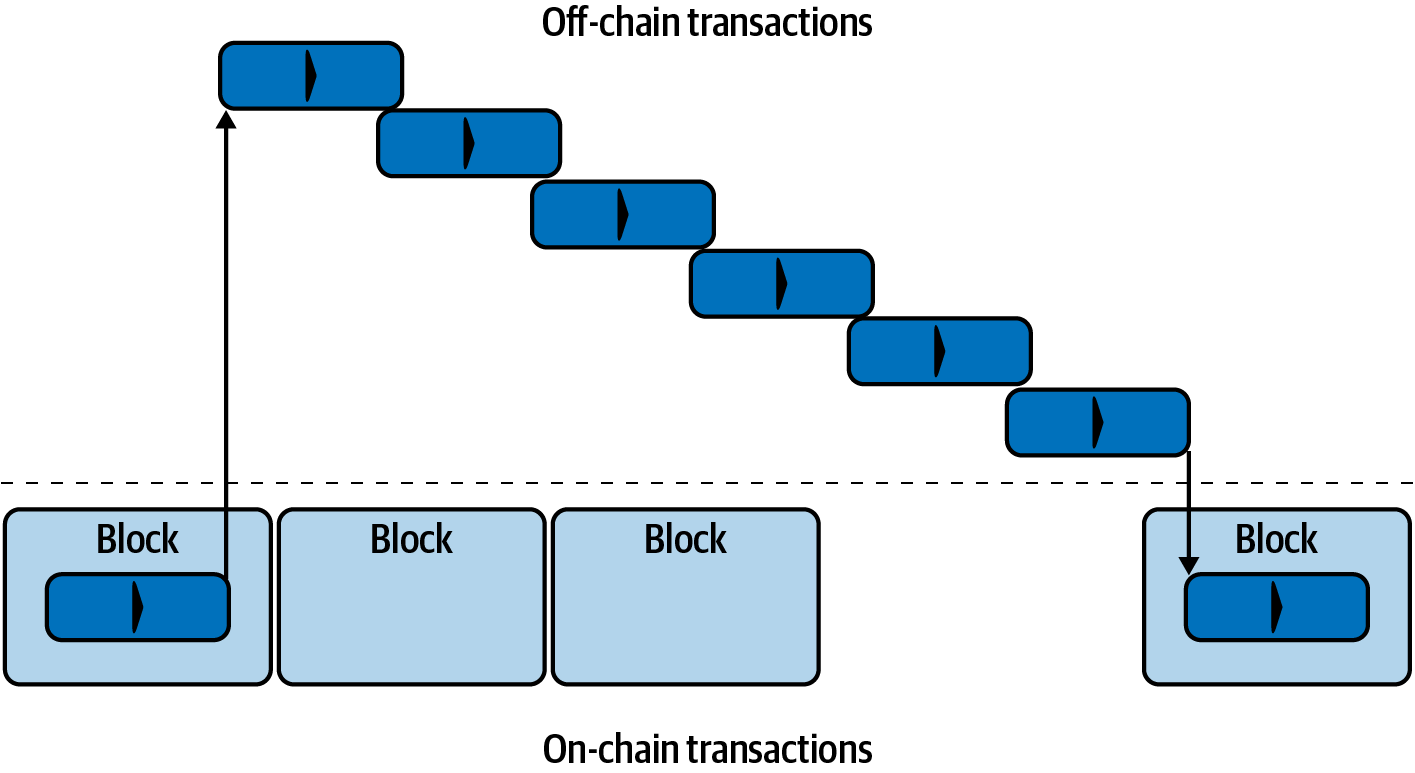
\includegraphics[width=0.6\columnwidth]{imgs/mtln_0702.png}
  \end{center}
    \caption{Diagram provides an overview of how the open and close a channel operations work~\cite{lnbook}.}
  \label{fig:ln-onchain}
\end{figure}


\begin{figure}[h]
  \begin{center}
  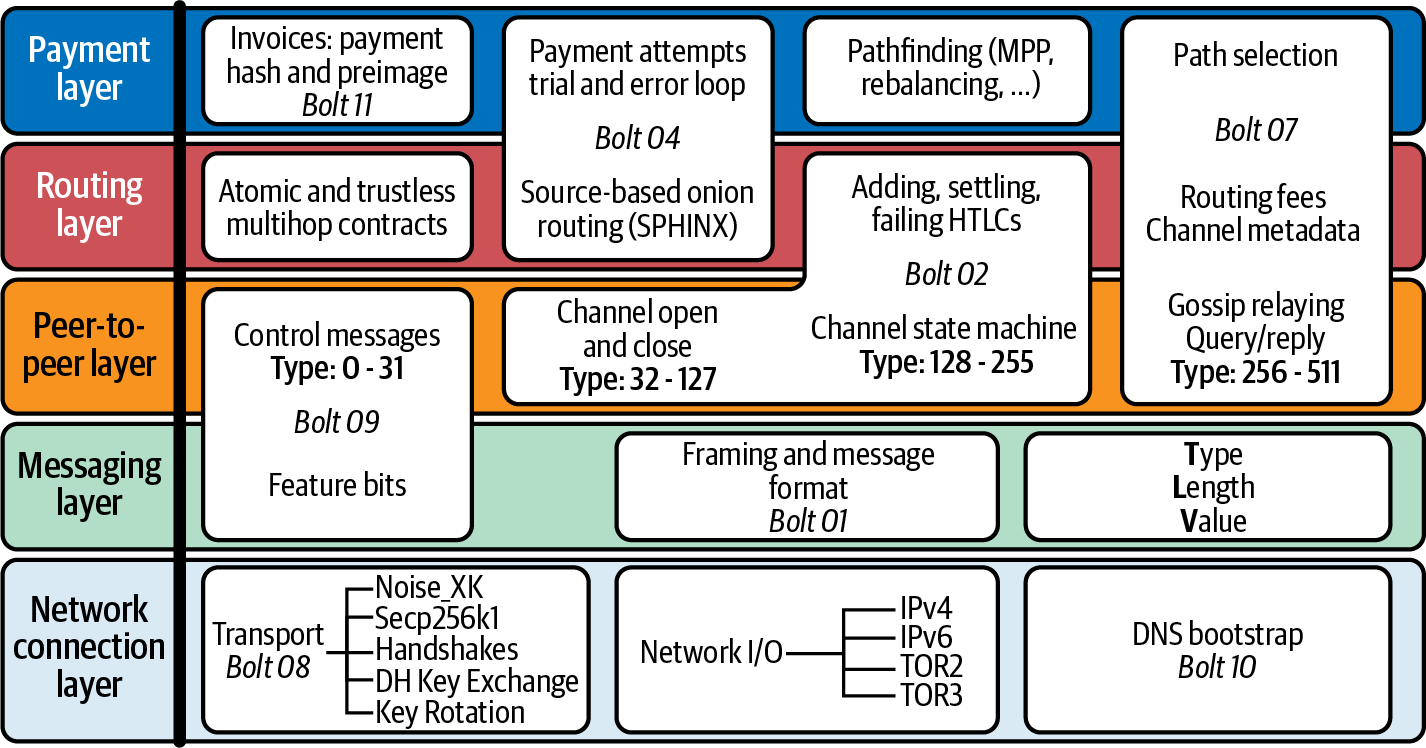
\includegraphics[width=0.6\columnwidth]{imgs/mtln_0601.png}
  \end{center}
    \caption{Diagram provides an overview of these layers and their component protocols~\cite{lnbook}.}
  \label{fig:lightning-stack}
\end{figure}

In the following Section there is described a general overview of how the {\LN} is implemented through the
\emph{BOLT} specification.\footnote{BOLT: Basis of Lightning Technology ({\LN} Specifications).}

\subsection{{\LN} Specifications}

Since 2016 the {\LN} began to be implemented by different teams,
and due the high overview of the {\LN} state machine definition in ~\cite{lightning-network-paper},
the implementations start to cooperate in a Specification that all the lightning implementations agree on.

The specification describes the following concepts to allow full interoperability between implementations:

\begin{itemize}
  \item BOLT 1: it describes the basics of the protocol, like how a message is encoded and what type of messages are required in order to support the communication;
  \item BOLT 2: it describes the peer-to-peer protocol for channels managements. This is one of the core concepts of lightning; indeed,  after a payment channel
        is settled up, the channels can have different cases that are described in the Section \ref{sec:channel_state}
  \item BOLT 3: it describes how the Bitcoin script language is used to compose the
        payment channel, and what kind of Bitcoin transactions are involved.
  \item BOLT 4: it describes the onion routing protocol that it is used to exchange messages between peers which in this case are called \emph{hops}.
        The routing schema is based on the \emph{Sphinx}~\cite{sphinx} construction and is extended with a per-hop payload.
  \item BOLT 5: it describes how the on-chain transaction should be handled.
  \item BOLT 7: it describes how the peer-to-peer node and channels are discovered through the network;
  \item BOLT 8: it describes all the authenticated and encrypted transport protocols;
  \item BOLT 9: it describes how the feature flags\footnote{Feature flags that are used to establish what kinds of feature are supported by a node} need to be managed;
  \item BOLT 10: it describes the DNS Bootstrap and Assisted Node Location;
  \item BOLT 11: it describes the invoice protocol for the {\LN} protocols.
\end{itemize}

%To add a new feature to the protocol it needs to be discussed between implementations and when at least two implementations support the feature, it is considered standard.\\
The actual implementations that are compliant and contribute to the {\LN} specification are:

\begin{itemize}
  \item \emph{core lightning}: it is the first implementation written in C, and it is written
        to be an efficient solution for servers. In addition, it is focused on improving the {\LN} specification. Indeed, core lightning has several new extensions such as the \emph{BOLT 12}\footnote{BOLT 12 is a new proposal to perform
        lightning payments and improve several problems that exist in the BOLT 11.} feature implemented and under discussion to be
        included in the standard protocol;
    \item \emph{lnd}: a {\LN} implementation written in Go lang. It is one of the most used {\LN} implementations according to ~\cite{lngossip};
  \item \emph{ldk}: a {\LN} implementation written in rust, that provides the lightning building blocks exposed as Library;
  \item \emph{eclair}: a {\LN} implementation written in Scala, widely used on mobile wallets, but supporting server side execution too.
\end{itemize}

\section{{\LN} Channel Operation}
\label{sec:channel_state}

The channel state management defines the state machine of the channels, and it is described in the BOLT 2 specification. It is a very complex
state machine where there are involved several steps in order to avoid bad
situations where a node can steal funds or lock the funds involved in the blockchain for a long period.\\
In this section we will provide a deep introduction to the primary operations to create and manage channels.

\subsection{Channel Establishment}
\label{sec:open_a_channels}

Opening a channel between two peers involves several steps before arriving at the point to construct the Bitcoin transaction also
known as \emph{funding transaction}.
In fact, the {\LN} protocol requires some connection steps between the two peers start to open a channel, this
operation is defined inside the BOLT 2~\cite{bolt2} as \emph{Channel Establishment}.

For this reason, each public peer is exposed to one or more public IP addresses where
they are listening for incoming connections, and when a peer wants to open
a channel with a specific peer the following information must be provided:

\begin{itemize}
  \item Node ID: It is the node's public key, differently from Bitcoin in this case it is public and it is one of the information included inside the gossip by the node;
  \item Node IP address and port: Where the node is listening for an incoming connection.
\end{itemize}

In addition, most of the nodes support the Tor network, but with the current usage of the protocol the Tor network provides very unreliable
performance as discussed in Section (TODO point to the problem Section).\\
After the node is connected with the counterpart, the Channel Establishment can be performed, and a sequence
of messages is exchanged (Figure \ref{fig:channel-establishment}). During this process
the following protocol messages are involved:

\begin{itemize}
  \item {\bf open\_channel}: The node that wants to open a channel (sender) creates an open channel message were the information of the
        Blockchain Network are defined (It is not required that this network need to be the Bitcoin network);
  \item {\bf accept\_channel}: The node that receives the open channel request (receiver) with the information of the Blockchain network to use
        can accept the request to open a channel by sending an accept channel message that contains the Blockchain network information, and
        a \emph{temporary\_channel\_id} generate from the peer information.
  \item {\bf funding\_created}: The sender after receiving the confirmation that the counterpart is ready to open a channel
        send a funding created message with the initial information of the funding transaction created as described in Section \ref{sec:htlc_intro}
  \item {\bf funding\_signed}: After the sender communicate the initial information for the funding transaction, the
        the receiver can send the signature for the \emph{refund transaction}\footnote{signature that allows the counterpart to claim her bitcoin back in case of protocol violation.} through a funding signed message, and at this moment the temporarily
        channel id sent in the previous steps can be overridden by a real channel id generated from the funding transaction information.
  \item {\bf funding\_lock}: The sender after committing the transaction on-chain can send a message funding lock to the counterpart when
        the on-chain transaction has reached enough confirmation. This message is also known as \emph{channel\_ready} message in the BOLT 2~\cite{bolt2}.
\end{itemize}

\begin{figure}[h]
  \begin{center}
  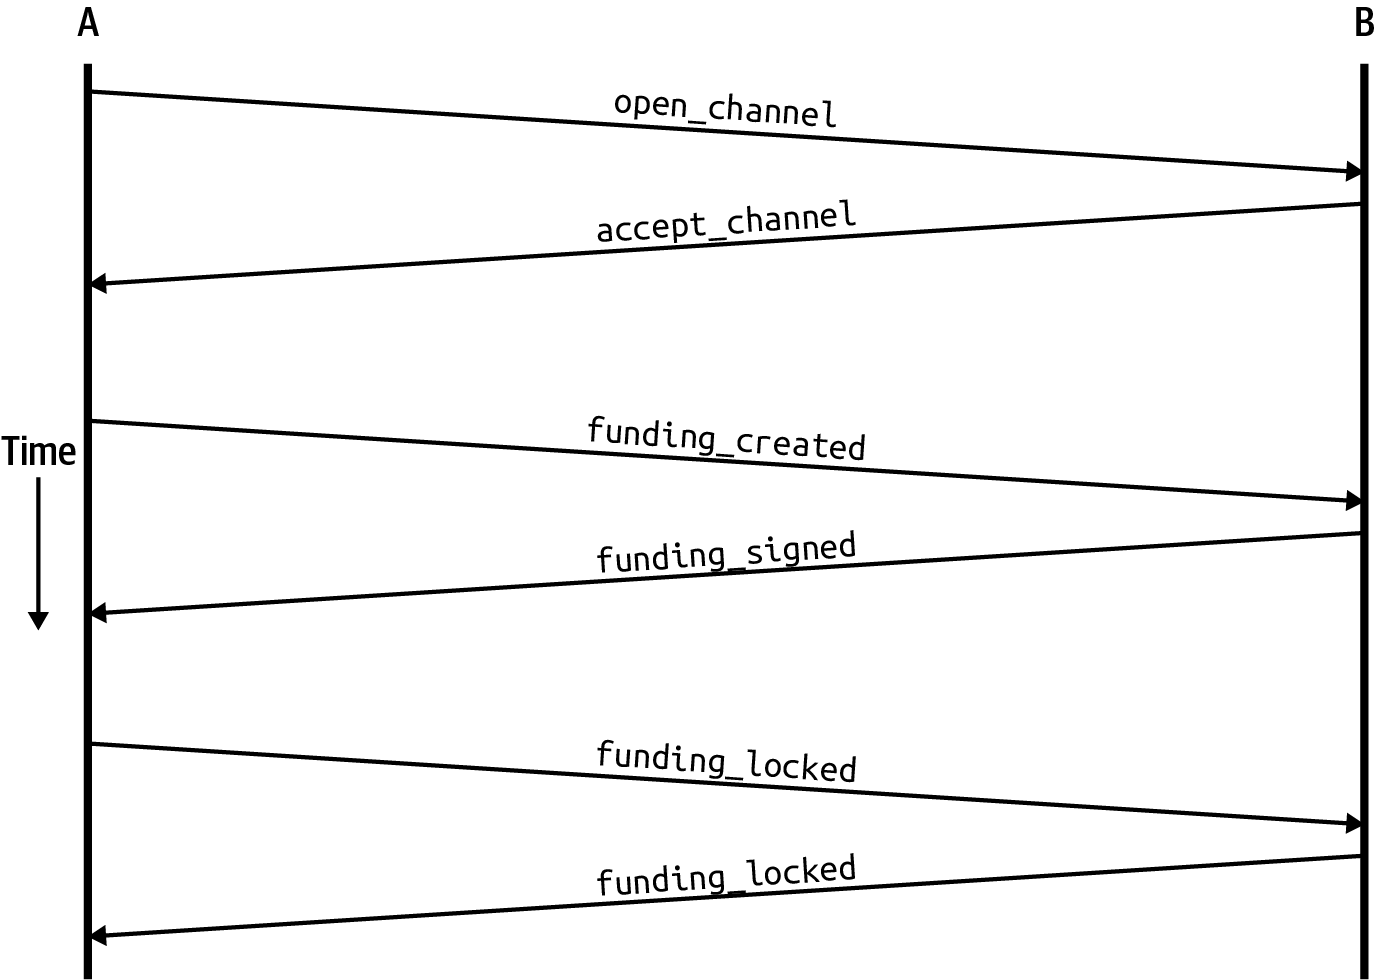
\includegraphics[width=0.6\columnwidth]{imgs/mtln_0703.png}
  \end{center}
    \caption{Channel Establishment procedure workflow.~\cite{lnbook}}
  \label{fig:channel-establishment}
\end{figure}

After the funding transaction is confirmed on the blockchain and the channel is ready to be used (this state of the channel is also known as \emph{normal state}),
peers can perform lightning payments that can modify the state of the current channel, in Section \ref{sec:modify_channel_state} is described how
these operations are performed inside the protocol.

\subsection{modifying Lightning Channel State}
\label{sec:modify_channel_state}

The {\LN} protocol complexity with the current implementation (defined in ~\cite{lightning-bolts})
is generated from the channel state management that needs to ensure that there are no situations that can
cause  possibilities to lose funds from one participant.
In fact, if one peer has an outdated channel state, and this state is shared with the network, the counterpart can
detect this inconsistency between the real channel state and the one received. In this case, the peer can and must
% FIXME: define the penality mechanism, but how?
perform the a \emph{penality mechanism} defined in the BOLT2~\cite{bolt2}, where the channel between the two peers
is closed and the receiver of the outdated channel state takes all the currency involved.\\
However, this penalty operation may be performed on peers that have bugs in the software and publish an old state of the
channel due to a corrupted database. In this case propose like ~\cite{eltoo} described in Section \ref{sec:eltoo} offers
better solutions for channel state management.

\subsection{Forwarding Lightning Payments}
\label{sec:lightning_forwarding}

The {\LN} protocol allows operations through the network by sending a partial sign transaction that
allow peers to perform a payment.
Therefore, in order to perform a payment the state of the channel needs to be altered, and in some cases the payment can involve
different peers long a \emph{route path}.\\
In fact, it is possible to send a payment to a peer directly connected with a channel, and send a payment to a peer
that is not directly connected. In the latter case, the peer needs to execute a routing algorithm
to find one of the best paths to reach the target peer.

When the route is found the payment can be sent across the channel or channels found by the routing algorithm, and this procedure
required to redistribute the balance of the channels involved in the payment process.\\
Therefore, when the channel is opened as discussed in the section \ref{sec:open_a_channels} the full channel balance
is distributed to the opener side\footnote{There is a proposal called \emph{dual funding channel} that allows the peers to open a channel
  with the balance distribute across both direction},
and payment is possible only from $Opener \rightarrow Receiver$ but not vice-versa. For this reason, to change the amount distribution
of the channel the sender sends a partially signed transaction to the receiver with the new information about the balance.
This update transaction is also known as \emph{commitment transaction}\footnote{A commitment transaction is also known as Hash Time Lock Contract (HTLC)} and in the Section \ref{sec:htlc_intro} is discussed how it is composed.
Figure \ref{fig:commitment_transaction_example} shows a possible commitment transaction workflow.

\begin{figure}[h]
  \begin{center}
  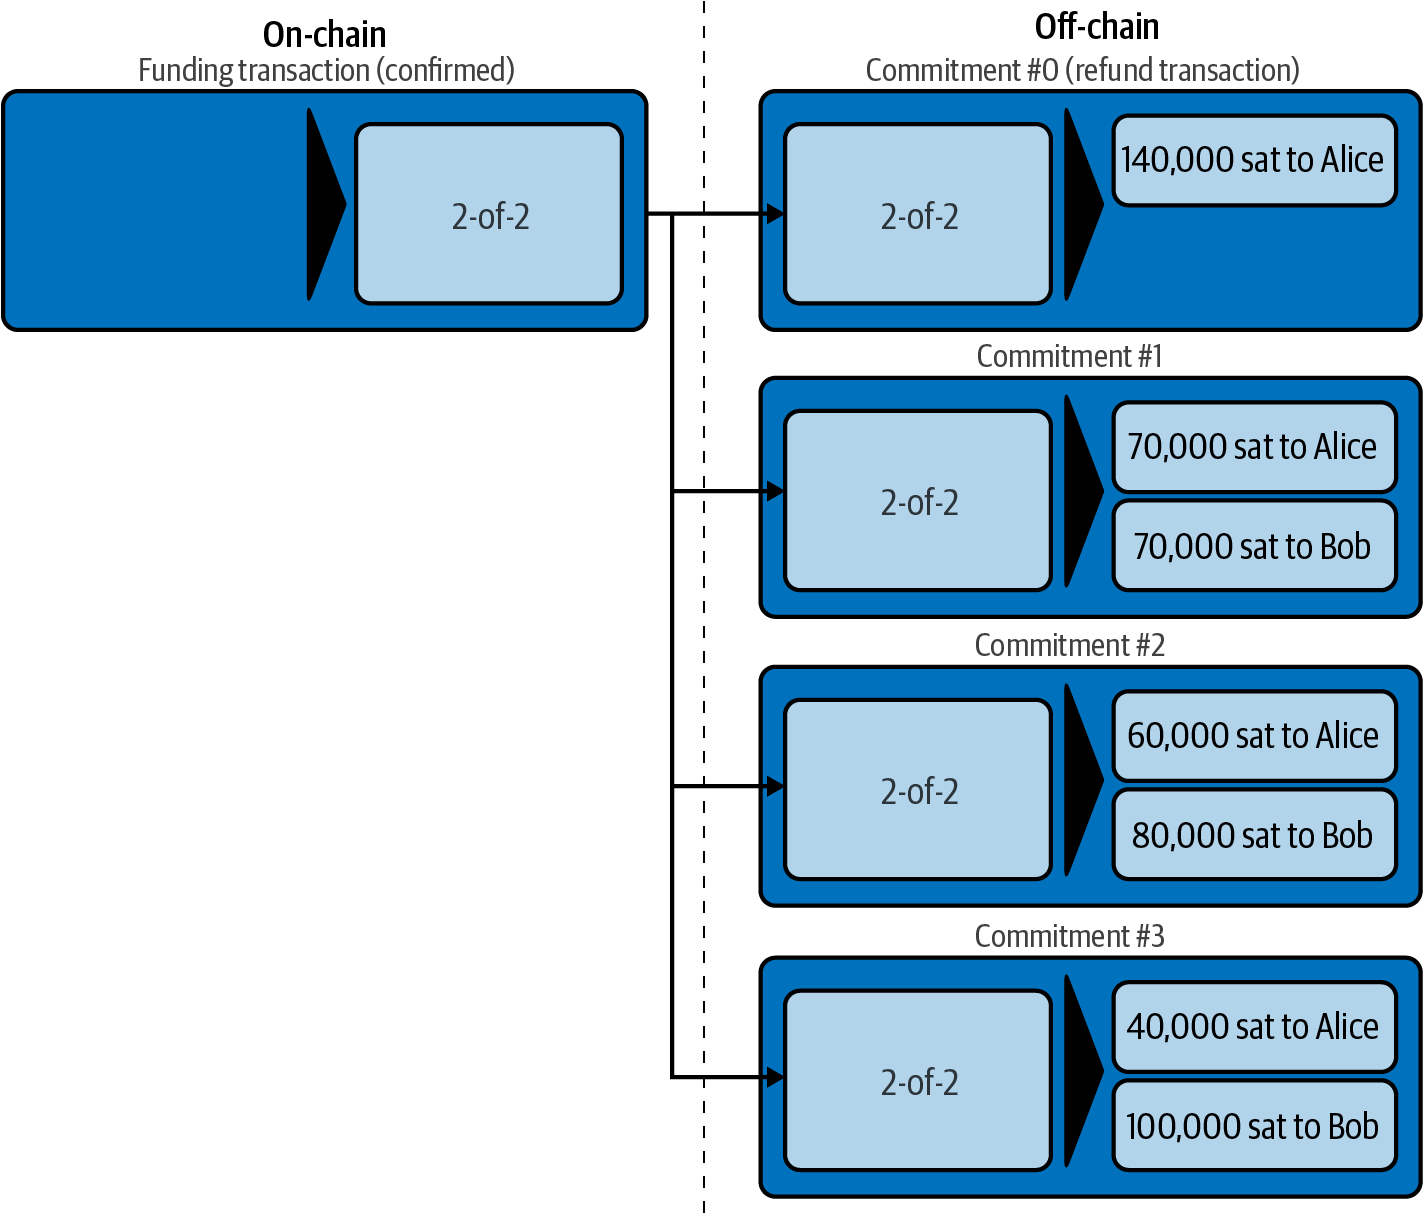
\includegraphics[width=0.6\columnwidth]{imgs/mtln_0706.png}
  \end{center}
    \caption{Commitment Transaction workflow example~\cite{lnbook}.}
  \label{fig:commitment_transaction_example}
\end{figure}


To perform the commitment transaction operation a sequence of {\LN} message are involved as shown in Figure \ref{fig:commitment_transaction_ln_messages}, and they are:

\begin{itemize}
  \item {\bf update\_add\_htlc}: When the sender wants to modify a channel and send a payment to the counterpart, it needs to send a message with the information of the channel that needs to be modified and including the new amount. In addition, this message includes
  the information regarding the onion rooting packet (Section \ref{sec:onion_routing});
  \item {\bf commitment\_signed}: The received of the update\_add\_htlc message confirms the operation by sending the signature for the new commitment transaction;
  \item {\bf revoke\_and\_ack}: The sender that received the signature of the new commitment transaction as confirmation of the update received. This message contains the revocation key of the sender to release the old commitment transaction, and the new information to construct the new revocation key, at this point the old commitment transaction is revoked.
  \item {\bf commitment\_signed} and {\bf revoke\_and\_ack}: The receiver if the revoke message, the operation of revocation is performed in the opposite direction where the receiver begins the sender and vice-versa.
  \item {\bf update\_fulfill\_htlc}: This message is sent back to the sender to confirm that the payment is received,
      % FIXME: define the payment preimage here!
      be the counterpart, and to prove that the receiver send this message that contains the \emph{payment preimage} 
        that is used to verify the payment hash. The payment preimage is used as proof or payment\footnote{clarify the payment preimage workflow and where this payment is made.}
\end{itemize}


\begin{figure}[h]
  \begin{center}
  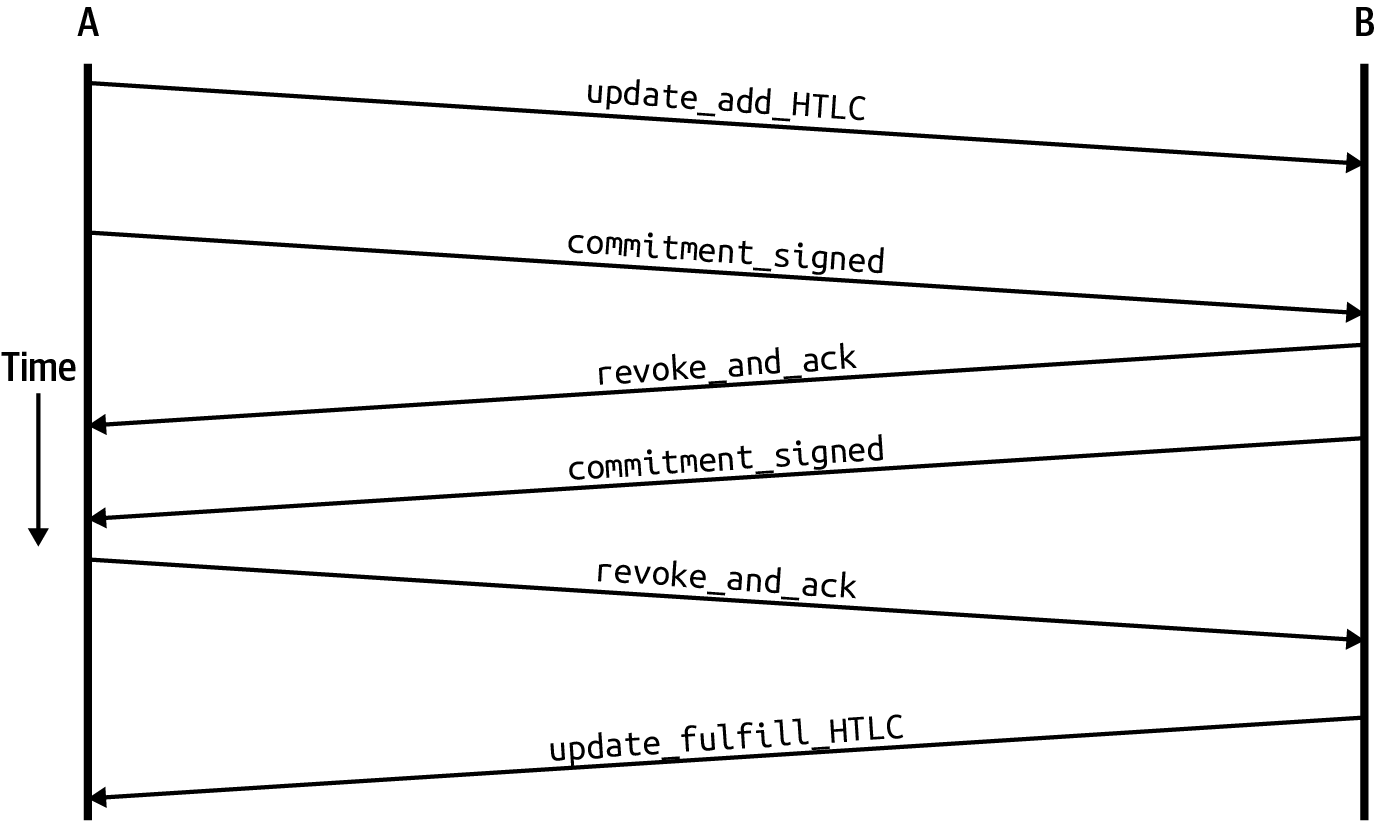
\includegraphics[width=0.6\columnwidth]{imgs/mtln_0903.png}
  \end{center}
    \caption{{\LN} protocol messages involved during a commitment transaction~\cite{lnbook}.}
  \label{fig:commitment_transaction_ln_messages}
\end{figure}


\section{Close {\LN} Channel}
\label{sec:close_operation}

At the current status of the implementation, the {\LN} protocol provides different cases where a channel can be closed such as:

\begin{itemize}
  \item Co-operative Closing: The channel parties arrive to an agreement where the channel can be closed and the
        \emph{closing transaction} (Section \ref{sec:htlc_intro}) can be broadcasted on the blockchain and the funds involved released.
  \item Unilateral Closing: One of the channel parties start to be unresponsive due to some problem, such as a technical problem, and the counterparty
        decided to force close the channel.
  \item Closing operation caused by penalty: There are corner cases briefly mentioned in \ref{sec:modify_channel_state} where a peer can voluntarily or involuntarily try to cheat the other party by publishing an old commitment transaction. In this case, the protocol provides a penalty mechanism to identify the cheat tentative and protect the party by closing the channel and moving all the balance of it to the peer that was undergoing the attack.
\end{itemize}

Section \ref{sec:modify_channel_state} is described how the state of the channel is modified, and it is described what kind of information is
exchanged between the peers. In particular, the peers have all the necessary information to broadcast on the blockchain an old commitment transaction.

For this reason, the protocol contains a sequence of option with a penalty where the node that will publish the old commitment transaction
will receive a punishment operation that involves losing funds. However, this is not the most common bad behavior that can happen in
the network, but it is possible that one of the peers begins unresponsive in the network for a period or forever, and the counterpart is forced to Unilateral close the channel. This operation
required that the funds are locked for an amount period, and it requires a much high on-chain fee cost for the peers involved.

\section{Onion Routing}
\label{sec:onion_routing}

In the {\LN}, it is used onion routing to forward payments through a specific path.
In particular, it is used a \emph{Source Base Rooting} where the payment path it is specified by the sender.
The goal of using the source base routing is to preserve privacy along the path. For this reason, a peer that
is forwarding a payment is able to know only the previous hop and the next hop, but there isn't any information
about the sender or recipient of the payment.

This section contains only an introduction a high overview of how onion routing works,
and how it is used in the {\LN} to forward HTLCs.

\subsubsection{Onion Routing Basics}

The base concept of onion routing is to build a packet in layers, where each peer can access only to the
first onion-encrypted layer. The layer is encrypted with the node, so only the owner of the layer can access to it.
The example \ref{ex:onion_routing} describes how the onion routing works across a routing path.

\begin{example}
  \label{ex:onion_routing}
  Consider that Alice wants to pay Dina with a Lightning Payment across a routing path generated as Figure \ref{fig:routing_path} shows.
  In particular, the routing packet built from Alice contains all the
  information to reach the Destination, across a pre-calculated path.
  In addition, it also shows how each peer has access only to the first layer (envelope in the figure) where it is possible to extract the information to the next hop.
  The current peer is also unable to understand if the next hop is the destination or if the previous hop is the source of the payment.

  {\centering
    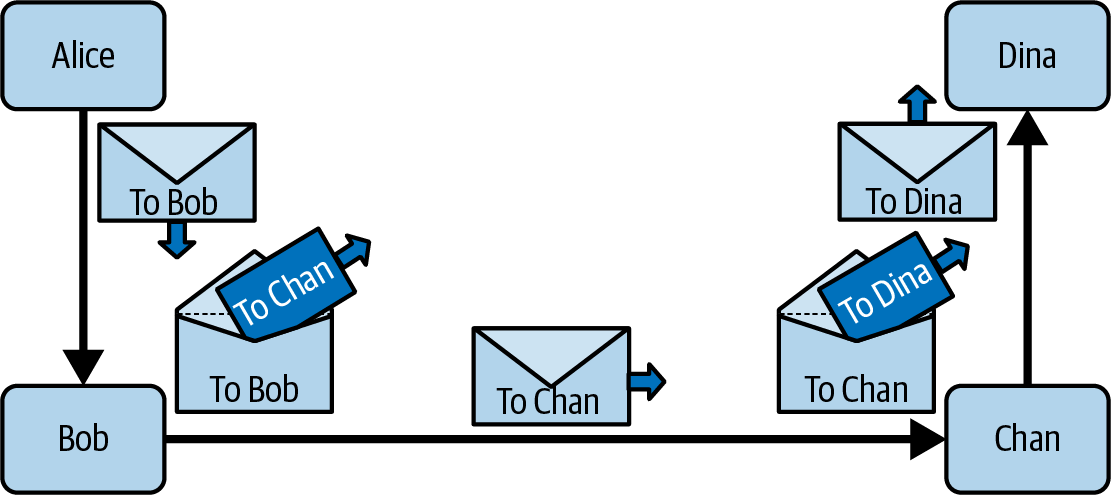
\includegraphics[width=0.6\columnwidth]{imgs/mtln_1007.png}
    \captionof{figure}{Onion Routing example to perform a payment from Alice to Dina~\cite{lnbook}.\label{fig:routing_path}}
    \par}
\end{example}

\subsubsection{Onion Routing with HTLCs}

{\LN} protocol implements a custom version of the Onion Routing based on Sphinx ~\cite{cryptoeprint:2008/475}. In this case the onion routing
the goal is to forward HTLC from the Source to the Destination and pay the fee to
every single hop by modifying the amount forward the next hop.

Therefore, a extension of the example\ref{ex:onion_routing} shows how
the HTLC forward with onion routing works.

\begin{example}
  \label{ex:htl_onion_routing}
  Consider that Alice wants to pay Dina with a Lightning Payment, and Alice had all the
  information that needs inside the \emph{gossip map}\footnote{The gossip map is a data structure that contains all the information that is gossiped through the network for each node. It is also known as Graph of the Network.} to feel the
  onion packet by including the fee that each peer is required to forward a payment
  along the pre-calculated path. Figure \ref{fig:routing_path_htlc} shows each node receives the HTLC with
  amount $X$ and forward the packet to the next hop with an amount $x - node_{fee}$

  {\centering
      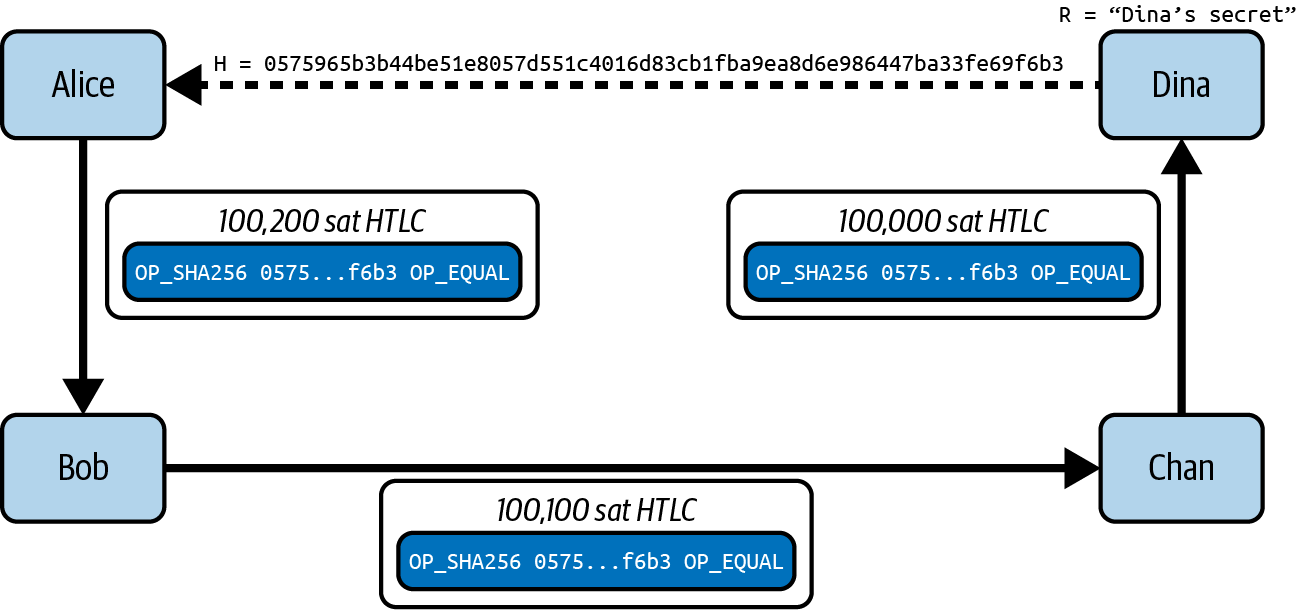
\includegraphics[width=0.6\columnwidth]{imgs/mtln_1008.png}
      \captionof{figure}{Onion Routing with HTLCs example to perform a payment from Alice to Dina.\label{fig:routing_path_htlc}}
  \par}  
\end{example}

The onion routing with HTLCs works pretty well in theory but the {\LN}
specification restricts (in order to preserve privacy) the information regarding
the channels balance for each node through the network, so the value
propagate is the total amount of Bitcoin that is involved in opening a channel as described in \ref{sec:open_a_channels}.

Therefore, in the example \ref{ex:htl_onion_routing} Alice has no idea if the current balance of the channel can support the payment amount\footnote{As described in the Section \ref{sec:open_a_channels} when a node opens a channel the amount of Bitcoin is distributed all in one side}, and in order to mitigate this limitation of information, there is an unofficial payment technique called \emph{multi path payment} that split a single payment into chunks and share each chunk across the different path.

\section{{\LN} Extension}
\label{sec:eltoo}

{\bf This need to be rewritten, because the current section is based on a blog post that was not clear at all, in fact this section do not make sense.}

By design, the current {\LN} protocol has to deal with punishment operations due to some wrong behavior or software error. For this reason, in order
to find a solution to this problem and simplify channel management different solutions have been proposed.
In this section, the Eltoo~\cite{eltoo} solution proposed by Christian Decker, Rusty Russell, and Olauluwa Osuntokun in April 30, 2018 is discussed.

Eltoo is based on top of BIP 118 ~\cite{bip118} also known as \emph{SIGHASH\_NOINPUT} that introduced semantics change inside the Bitcoin Scrip language\footnote{Bitcoin Scrip is the language to describe smart contract on the Bitcoin blockchain.}, and turn the {\LN} protocol to a no penalty base protocol.
Therefore in this case the two parties create the funding transaction denoted by \emph{Setup} in Figure \ref{fig:eltoo_diagram_tx}.

\begin{figure}[h]
  \begin{center}
    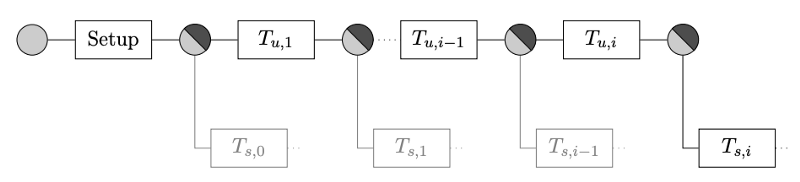
\includegraphics[width=0.6\columnwidth]{imgs/1_USwvkUzr2-EHHkImnYz6gw.png}
  \end{center}
  \caption{Eltoo transaction diagram ~\cite{eltoo}.}
  \label{fig:eltoo_diagram_tx}
\end{figure}


In addition, before ~\cite{Palazzo_Estrazione_di_Informazioni_2019} need to sign a refund transaction called \emph{settlement transaction} which refunds the funding transaction back to the owner (this is possible with the BIP 118~\cite{bip118} proposal), and the Bitcoin script is described in the Section \ref{sec:eltoo_htlc}.

In conclusion, the proposal drastically simplify the {\LN} Protocol, but for the moment there is no implementation of it.
